\section{\bf Scientific Background}

\subsection{Introduction}

Since the theory of context-free grammars was developed by Noam Chomsky, it has been extensively studied~\cite{chomsky1959certain,chomsky1963algebraic}. The classic application of context-free grammars is describing natural and programming  languages. Recent  research has  shown  that the theory of formal languages and, in particular, context-free languages can be used in bioinformatics~\cite{rivas,knudsen,yuan,dowell}.

A good example of this usage is the recognition and classification problems in bioinformatics, some of them are based on the research claiming that the secondary structure of the DNA and RNA nucleotide sequence contains important information about the organism species. The specific features of the secondary structure can be described by some context-free grammar, and therefore the recognition problem can be reduced to parsing---verification if some nucleotide sequence can be derived in this grammar.
%That means we try to find the substrings in DNA or RNA sequences possessing these specific features and further we can draw conclusions about the organism's origin based on the availability and location of the found substrings.

Such field of application as bioinformatics requires working with a large amount of data, so it is necessary to find highly efficient parsing algorithm. Moreover, this algorithm needs to be easily adaptive to such computing techniques as GPGPU (General-Purpose computing on Graphics Processing Units) or CPU parallel computing which is now a fairly widespread method to accelerate the computation.

The majority of parsing algorithms either has the cubic-time complexity (Kasami~\cite{Kas}, Younger~\cite{Younger:1966:CLP:1441427.1442019}, Earley~\cite{Earley:1970:ECP:362007.362035}) or could work only with sub-classes of context-free grammars (Bernardy, Claussen~\cite{Bernardy:2013:EDP:2544174.2500576}), but still asymptotically more efficient parsing algorithm that can be applied to any context-free grammar is algorithm based on matrix multiplication proposed by Leslie Valiant~\cite{Valiant:1975:GCR:1739932.1740048}. It computes the parsing table for a linear input, where each element of this table is responsible for deriving a particular substring. By offloading the most time-consuming computations on a Boolean matrix multiplication, Valiant has achieved an improvement in time complexity, which is O(BMM(n)log(n)) for an input string of size n, where BMM(n) is the number of operations needed to multiply two Boolean matrices of size n $\times$ n. In addition, Okhotin generalized the matrix-based algorithm to conjunctive and Boolean grammars which are the natural extensions of context-free grammars with more expressive power and also improved its performance and understandability~\cite{Okhotin:2014:PMM:2565359.2565379}. In spite of the fact that Valiant's algorithm allows us to use parallel techniques, for example, compute matrix products on GPUs, it seems like a large part of matrix multiplications can be performed concurrently.

In this paper, we show how to reorganize the matrix multiplication order in Valiant's algorithm to divide the parsing table into successively computed layers of disjoint submatrices where each submatrix of the layer can be processed independently.

We make the following contributions:
\begin{itemize}
  \item We propose the modification of Valiant's algorithm which allows to compute some matrix products concurrently and improve the performance through parallel techniques.
  \item We prove the correctness of the modification and provide its time complexity estimation which is $O(|G|BMM(n)log(n))$ for an input string of length n, where BMM(n) is the number of operations needed to multiply two Boolean matrices of size $n \times n$.
  \item We show the applicability of our approach in bioinformatics research, especially in addressing the string-matching problem.
  \item We have implemented the proposed algorithm and our evaluation shows that ... parallel techniques improve the performance...
\end{itemize}


\subsection{Preliminaries}

An alphabet $\Sigma$ is a finite nonempty set of symbols. $\Sigma^{*}$ is a set of all finite strings over $\Sigma$.
A grammar is a quadruple $(\Sigma, N, R, S)$, where $\Sigma$ is a finite set of terminals, $N$ is a finite set of nonterminals, $R$ is a finite set of productions of the form $\alpha \rightarrow \gamma$, where $\alpha \in V^{*}NV^{*}$, $\gamma \in V^{*}$, $V = \Sigma \cup N$ and $S \in N$ is a start symbol.

Grammar $G = (\Sigma, N, R, S)$ is called context-free, if $\space\forall r \in R$ are of the form $A \rightarrow \beta$, where $A \in N, \beta \in V^{*}$.

Context-free grammar $G = (\Sigma, N, R, S)$ is said to be in Chomsky normal form if all productions in R are of the form:
\begin{itemize}
  \item $A \rightarrow BC$,
  \item $A \rightarrow a$,
  \item $S \rightarrow \varepsilon$,
\end{itemize}
where $A, B, C \in N, a \in \Sigma, \varepsilon$ is an empty string.

$L_{G}(A)$ is a language of the grammar $G_{A} = (\Sigma, N, R, A)$, which means all the sentences that can be derived in a finite number of rules applications from the start symbol $A$.

\subsection{Parsing by matrix multiplication}

The main problem of parsing is to verify if the input string belongs to the language of some given grammar $G$. We will describe the Cocke-Younger-Kasami algorithm and the most asymptotically efficient parsing algorithm, which works for all context-free grammars, Valiant's parsing algorithm, based on matrix multiplication. In this paper we use the rewritten version of Valiant's algorithm proposed by Alexander Okhotin.

The CYK algorithm is a basic parsing algorithm.
Its main idea is to construct a parsing table $T$ of size $(n + 1) \times (n + 1)$ for an input string $a_{1}a_{2} \dots a_{n}$ and context-free grammar $G = (\Sigma, N, R, S)$ which is in Chomsky normal form, where

$$T_{i, j} =  \{ A | A \in N, a_{i + 1} \dots a_{j} \in L_{G}(A)\} \quad \forall i < j.$$

The elements of $T$ are filled successively beginning with
$ T_{i - 1, i} = \{ A | A \rightarrow a_{i} \in R\}.$
Then, $ T_{i, j} = f(P_{i, j})$ where
$$ P_{i, j} = \bigcup\limits_{k = i + 1}^{j - 1} T_{i,k} \times T_{k, j}  $$
$$ f(P) = \{A | \exists A \rightarrow BC \in R : (B, C) \in P\} $$

The input string $a_{1}a_{2} \dots a_{n}$ belongs to $L_{G}(S)$ if and only if $S \in T_{0, n}$.

% Algorithm1
\begin{algorithm}[t]
\SetAlgoNoLine
\KwIn{Grammar $G = (\Sigma, N, R, S), w = a_{1} \dots a_{n}, n \geq 1, a_{i} \in \Sigma$, where  n + 1 is a power of two}
\underline{main()}{:}{

 \textit{compute(0, n + 1)\;}
 accept if and only if $S \in T_{0, n}$
 \linebreak
 }

\underline{compute(\textit{l, m})}{:}{

 \If {$m - l \geq 4$}{
     \textit{compute(l, $\frac{l+m}{2}$)\;
     compute($\frac{l+m}{2}$, m)}}
 \textit{complete(l, $\frac{l+m}{2}$, $\frac{l+m}{2}$, m)}
 \linebreak
 }

\underline{complete(\textit{l, m}, $l^\prime$, $m^\prime$)}{:}{

 \If {$m - l = 4$ and $m = l^\prime$}{$T_{l, l + 1} = \{A | A \rightarrow a_{l+ 1} \in R\}$\;}
 \ElseIf{$m - l = 1$ and $m < l^\prime$}{ $T_{l, l'} = f(P_{l, l'})$\;}
 \ElseIf{$m - l > 1$}{
    $leftgrounded = (l, \frac{l+m}{2}, \frac{l+m}{2}, m), rightgrounded = (l', \frac{l'+m'}{2}, \frac{l'+m'}{2}, m')$,

    $bottom = (\frac{l+m}{2}, m, l', \frac{l'+m'}{2}), left = (l, \frac{l+m}{2}, l', \frac{l'+m'}{2})$,

    $right = (\frac{l+m}{2}, m, \frac{l'+m'}{2}, m'), top = (l, \frac{l+m}{2}, \frac{l'+m'}{2}, m')$\;
    complete(bottom)\;
    $P_{left} = P_{left} \cup (T_{leftgrounded} \times T_{bottom})$\;
    complete(left)\;
    $P_{right} = P_{right} \cup (T_{bottom} \times T_{rightgrounded})$\;
    complete(right)\;
    $P_{top} = P_{top} \cup (T_{leftgrounded} \times T_{right})$\;
    $P_{top} = P_{top} \cup (T_{left} \times T_{rightgrounded})$\;
    complete(top)
    }
 }
\caption{Parsing by matrix multiplication: Valiant's Version}
\label{algo:valiant}
\end{algorithm}

The time complexity of this algorithm is $O(n^3)$. Valiant proposed to offload the most intensive computations to the Boolean matrix multiplication. As the most time-consuming is computing $\bigcup\limits_{k = i + 1}^{j - 1} T_{i, k} \times T_{k, j}$, Valiant rearranged computation of $T_{i, j}$, in order to use multiplication of submatrices of $T$.

\label{def:defn4} Let $X \in (2^N)^{m \times l}$ and $Y \in (2^N)^{l \times n}$ be two submatrices of parsing table $T$. Then, $X \times Y = Z$, where $Z \in (2^{N \times N})^{m \times n}$ and $Z_{i, j} = \bigcup\limits_{k = 1}^{l} X_{i, k} \times Y_{k, j}$.

In listing~\ref{algo:valiant} full pseudo-code of Valiant's algorithm is written in the terms proposed by Okhotin, is presented. All elements of $T$ and $P$ are initialized by empty sets. Then, the elements of these two table are successively filled by two recursive procedures. 

In figure~\ref{fig1} is presented a simple example of Valiant's algorithm. Only the beginning of the work is shown, because later we point out at this version and our approach differences. 

\begin{figure}
    \centering
    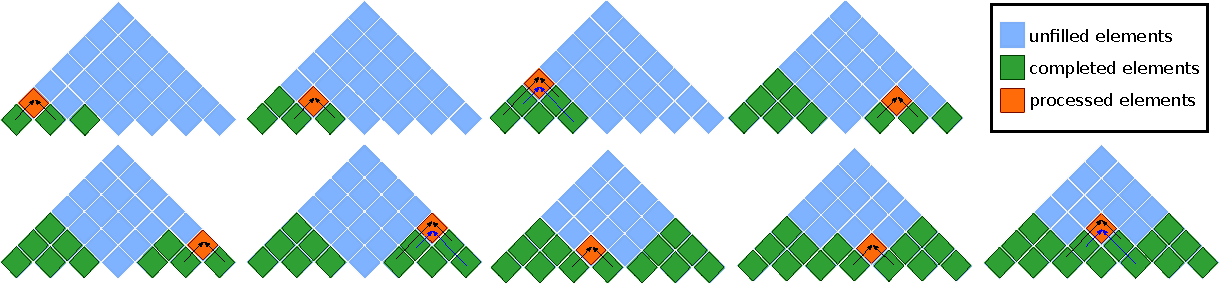
\includegraphics[width=0.900\textwidth]{pictures/valbeg2.pdf}
    \caption{An example of beginning of Valiant's algorithm}
    \label{fig1}
\end{figure}

The procedure $compute(l, m)$ constructs the correct values of $T_{i,j}$ for all $l \le i < j < m$.

The procedure $complete(l, m, l', m')$ constructs the submatrix $T_{i, j}$ for all $l \le i < m$, $l' \le j < m'$. This procedure assumes $T_{i, j}$ for all $l \leq i < j < m,  l' \leq i < j < m'$ are already constructed and the current value of  $P[i, j] =  \{ (B, C) |\exists k, (m \le k < l'), a_{i + 1} \dots a_{k} \in L(B), a_{k + 1} \dots a_{j} \in L(C)\}$ for all $l \leq i < m,  l' \leq j < m'$. The submatrix division during the procedure call is shown in figure~\ref{fig2}.

Then Valiant described that product of multiplying of two submatrices of parsing table $T$ can be provided as $|N|^2$ Boolean matrices (for each pair of nonterminals). Denote matrix corresponding to pair $(B, C) \in N \times N$ as $Z^{(B, C)}$, then $Z_{i, j}^{(B, C)} = 1$ if and only if $(B, C) \in Z_{i, j}$. It should also be noted that $Z^{(B, C)} = X^{B} \times Y^{C}$. So, matrix multiplication in definition~\ref{def:defn4} can be replaced by Boolean matrix multiplication, each of which can be computed independently. Following these changes, time complexity of algorithm in listing~\ref{algo:valiant} is $O(|G|BMM(n)log(n))$ for an input string of length $n$, where $BMM(n)$ is the number of operations needed to multiply two Boolean matrices of size $n \times n$.

\begin{figure}
    \centering
    \captionsetup{justification=centering}
    \begin{minipage}{0.40\textwidth}
        \centering
        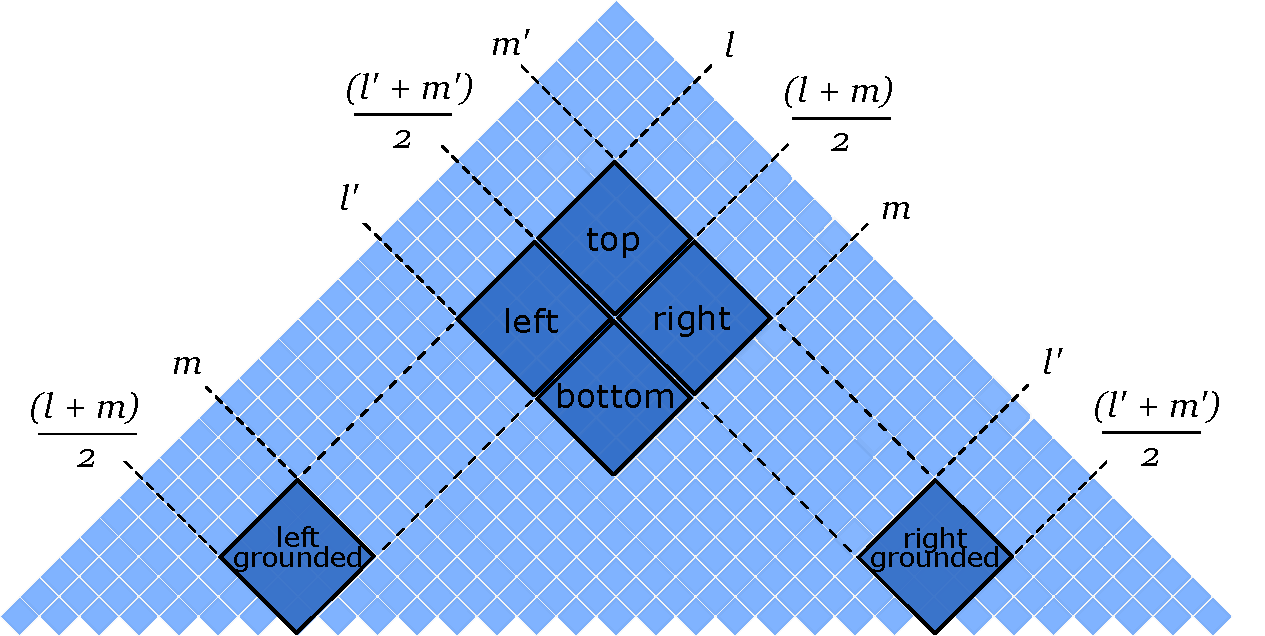
\includegraphics[width=1\textwidth]{pictures/splitting_with_grounded.pdf}
        \caption{Matrix partition used in \linebreak \textit{complete(l, m, l', m')} procedure.}
        \label{fig2}
    \end{minipage}\hfill
    \begin{minipage}{0.40\textwidth}
        \centering
        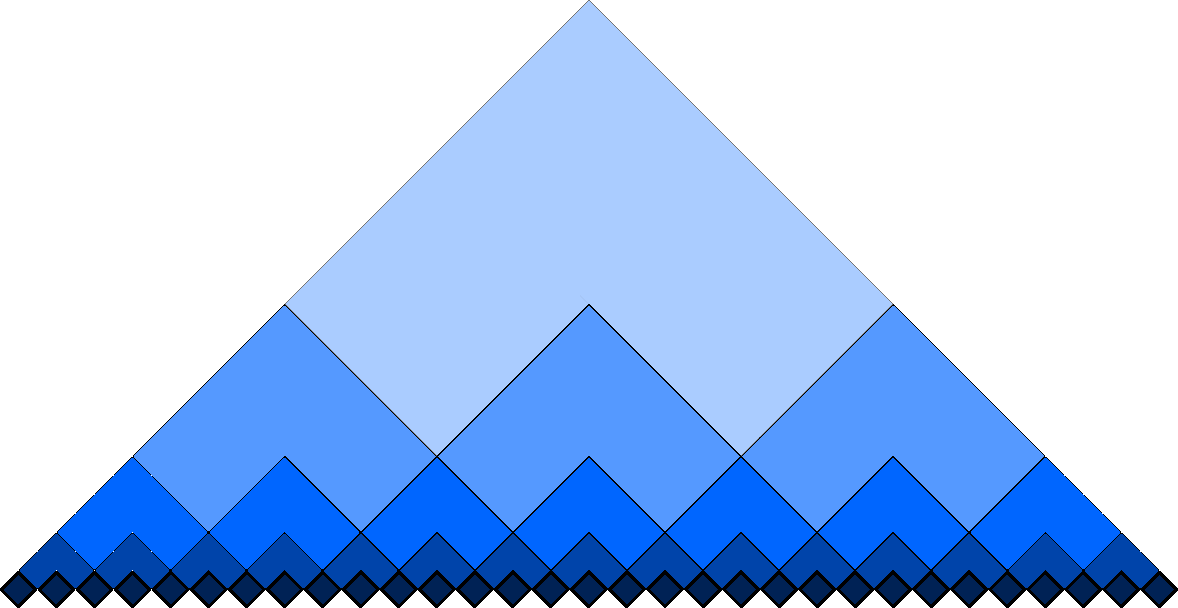
\includegraphics[width=1\textwidth]{pictures/layers.pdf}
        \caption{Matrix partition on V-shaped layers.}
        \label{fig3}
    \end{minipage}
\end{figure}